\documentclass{theme-2639013-final}
\usepackage{hyperref}
\usepackage{bookmark}
\usepackage{minted}

\usepackage{tikz}
\usetikzlibrary{positioning, shapes.geometric}

\usepackage{multicol}

% =============================================
% Part 0 信息
% =============================================

\mathsetup{
  % 学生姓名
  student-name = {某同学},
  % 学号
  student-id = {2021xxxx},
  % 院系
  department = {电子与信息工程学院},
  % 班级
  class = {2021391 班},
  % 专业
  experiment = {STM32 多功能计算器},
  % 专业年级
  major = {集成电路设计与集成系统},
  % 日期
  % date = {\today},
}

\begin{document}

% =============================================
% Part 1  封面
% =============================================

\makecover

% =============================================
% Part 2 主文档
% =============================================

\section{设计要求}

通过触摸屏实现一个简易的计算器,具有完整的多位加减乘除功能。

\section{设计思路}

\begin{enumerate}
  \item 在LCD屏幕显示计算器的界面设计。
  \item 在LCD屏幕底部显示当前时间和蜂鸣器是否启用。
  \item 通过触摸屏实现数字的输入和操作符的选择。
  \item 通过键盘实现数字的输入和操作符的选择。
  \item 通过按键中断设定输入时是否启用蜂鸣器。
  \item 编写程序实现计算器的功能。
  \item 通过LCD屏幕输出计算器的运算表达式。
  \item 通过串口输出计算器的运算结果。
\end{enumerate}

程序运行流程如下:

\begin{figure}[H]
  \centering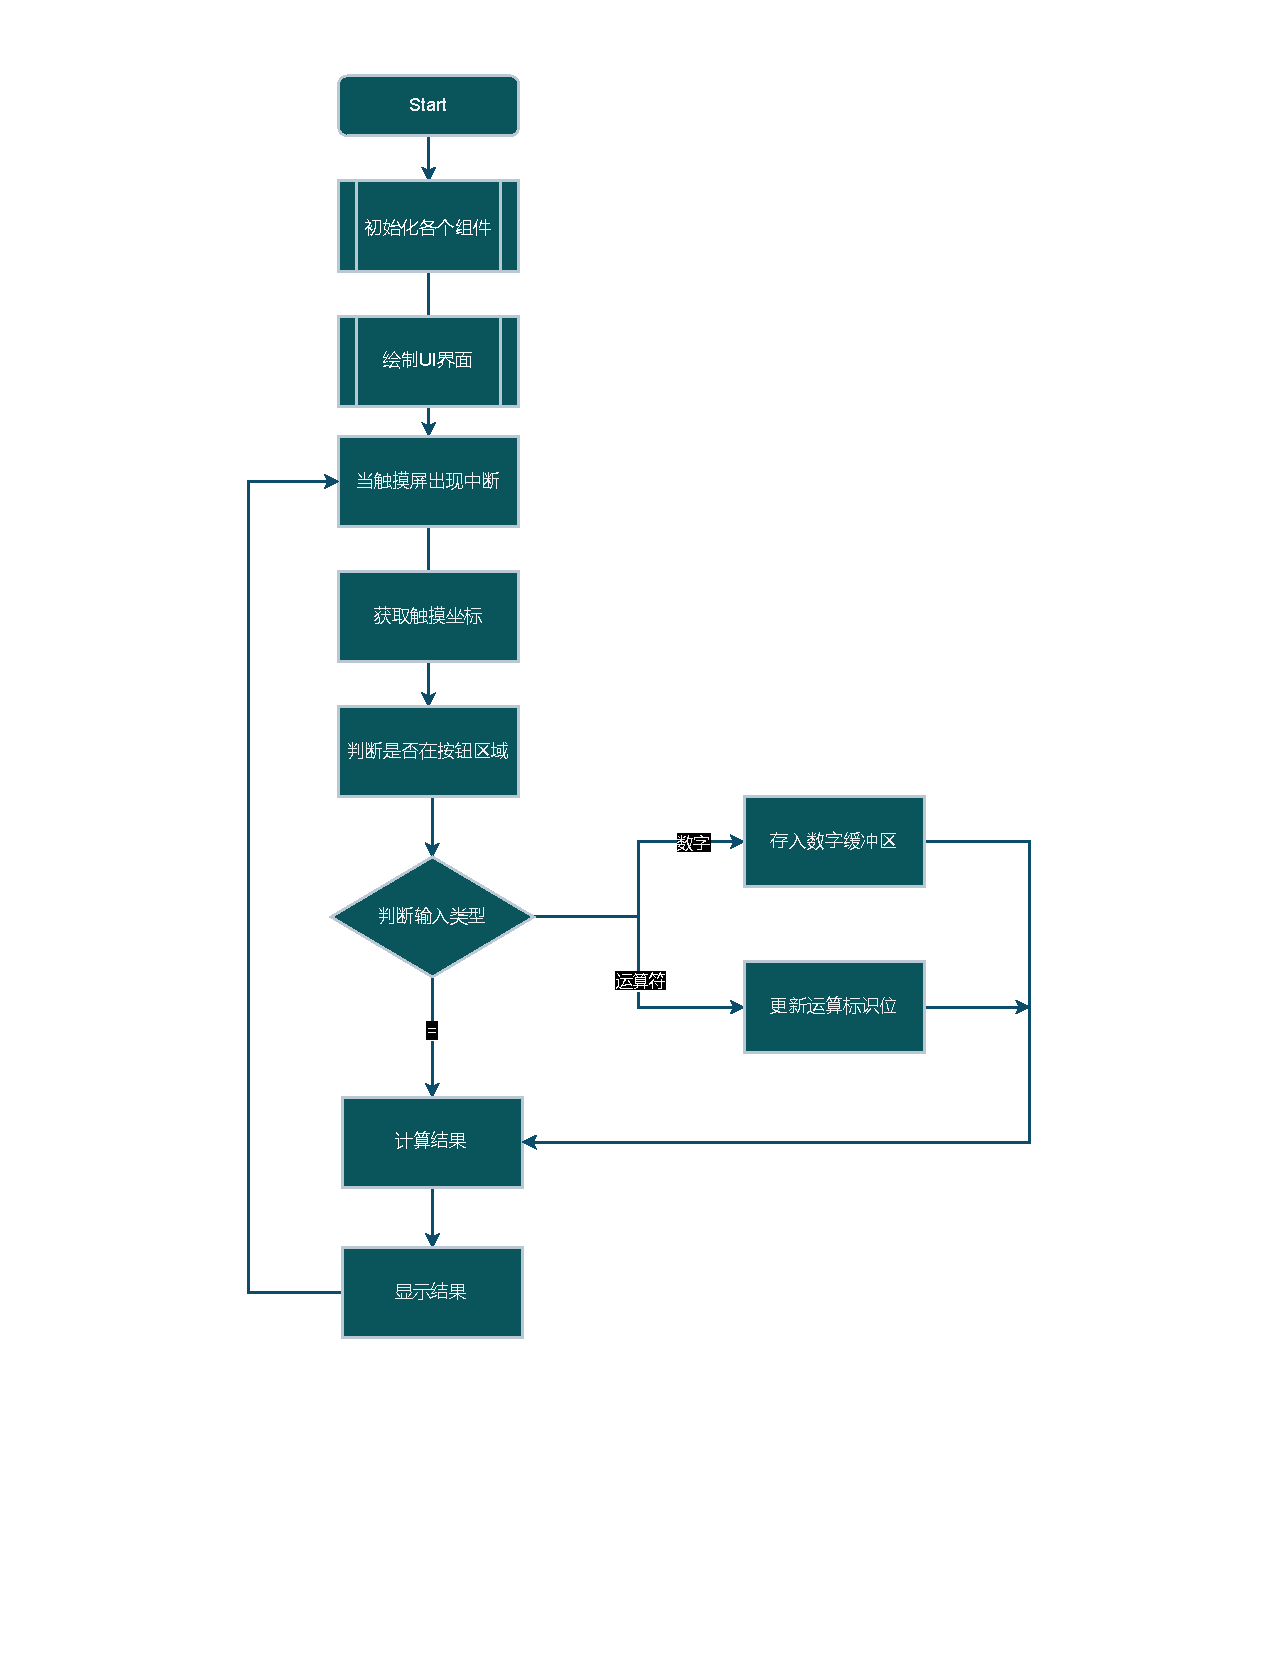
\includegraphics[width=0.7\linewidth]{flowchart.drawio.pdf}
  \caption{程序运行流程}
\end{figure}

% \begin{tikzpicture}[node distance=20pt]{center}
%   \node[draw, rounded corners]                        (start)   {Start};
%   \node[draw, below=of start]                         (step 1)  {初始化各个组件};
%   \node[draw, below=of step 1]                        (step 2)  {绘制UI界面};
%   \node[draw, below=of step 2]                        (step 3)  {当出现触摸屏中断};
%   \node[draw, below=of step 3]                        (step 4)  {获取触摸屏坐标};
%   \node[draw, below=of step 4]                        (step 5)  {判断触摸屏坐标是否在按钮区域};
%   \node[draw, below=of step 5]                        (input 1)  {将对应按键值传回主函数};
%   \node[draw, diamond, aspect=2, below=of step 2]     (choice)  {判断按键类型};
%   \node[draw, left=of choice]                         (case 1)  {数字};
%   \node[draw, right=of choice]                        (case 2)  {运算符};
%   \node[draw, below=of choice]                        (case 3)  {“=”};
%   \node[draw, below=of case 1]                         (step 6)  {将数字存入缓冲区};
%   \node[draw, below=of case 2]                         (step 7)  {将运算符存入缓冲区};
%   \node[draw, below=of case 3]                        (step 8)  {计算结果并清理中间变量};
%   \node[draw, below=of step 8]                        (step 9)  {显示结果};

%   % \node[draw, rounded corners, below=20pt of choice]  (end)     {End};
  
%   \draw[->] (start)  -- (step 1);
%   \draw[->] (step 1) -- (step 2);
%   \draw[->] (step 2) -- (step 3);
%   \draw[->] (step 3) -- (step 4);
%   \draw[->] (step 4) -- (step 5);
%   \draw[->] (step 5) -- (input 1);
%   \draw[->] (input 1) -- (choice);
%   \draw[->] (choice) -- node[left] (case 1);
%   \draw[->] (choice) -- node[right] (case 2);
%   \draw[->] (choice) -- (case 3);
%   \draw[->] (case 1) -- (step 6);
%   \draw[->] (case 2) -- (step 7);
%   \draw[->] (case 3) -- (step 8);
%   \draw[->] (step 6) -- (case 3);
%   \draw[->] (step 7) -- (case 3);
%   \draw[->] (step 8) -- (step 9);
% \end{tikzpicture}

\section{设计内容}

% 重点部分代码截图与解释
本项目使用了 STM32F4 微控制器,结合触摸屏、键盘、蜂鸣器、LED、RTC、USART、按键中断等功能,实现了一个简易的计算器。

\subsection{主函数}

\subsubsection{main}

主函数代码分析:

\begin{enumerate}
  \item 变量声明部分
    \begin{enumerate}
      \item \texttt{char input\_value;}: 用于存储用户输入的字符。
      \item \texttt{int key\_value = 0;}: 存储键盘输入的值。
      \item \texttt{double num = 0.0;} 和 \texttt{double result = 0.0;}: 用于存储数字和计算结果的变量,以双精度浮点数的形式。
      \item \texttt{int flag\_num = 0;}: 用于标记当前程序处于等待输入第一个数字还是等待输入第二个数字的状态。
      \item \texttt{int flag\_calc = 0;}: 用于标记当前计算器将执行的操作类型(加法、减法、乘法或除法)。
      \item \texttt{char input\_sequence[100] = ""}: 用于存储用户输入的数字和操作符的数组。
      \item \texttt{char display\_buffer[100] = ""}: 用于存储计算结果以及显示在LCD上的其他信息的数组。
      \item \texttt{int BeepFlag = 1;}: 用于控制蜂鸣器的状态。
    \end{enumerate}

  \item 主函数 \texttt{main()}
    \begin{enumerate}
      \item 进行了各种外设(LED、GPIO、BEEP、EXTI、RTC、USART等)的初始化配置。
      \item 初始化了LCD屏幕。
      \item 检查RTC备份寄存器,若未设置时间和日期,则进行设置。
      \item 初始化触摸屏,并根据液晶的扫描方向更新触摸配置。
      \item 绘制计算器界面。
      \item 进入了一个无限循环 \texttt{while (1)} 中,不断监听用户输入和触摸事件。
    \end{enumerate}

  \item 主循环部分
    \begin{enumerate}
      \item 不断检测触摸中断和键盘输入,并在有输入时执行相应的操作。
      \item 若触摸中断发生,则获取输入并处理,若 \texttt{BeepFlag == 1} 则同时开启蜂鸣器以示提示。
      \item 若键盘输入发生,则进行按键扫描。
      \item 通过 \texttt{Calculate()} 函数处理输入,计算结果并显示在LCD上。
      \item 循环显示当前输入的数字和操作符。
      \item 显示计算结果和当前时间。
    \end{enumerate}
\end{enumerate}

\begin{minted}[
  frame=lines,
  framesep=2mm,
  baselinestretch=1.2,
  fontsize=\small,
]{C++}
char input_value;
int key_value = 0;
double num = 0.0;
double result = 0.0;
int flag_num = 0;  // 0: waiting for first number, 1: waiting for second number
int flag_calc = 0; // 0: +, 1: -, 2: *, 3: /
char input_sequence[100] = ""; // 用于存储输入的数字和操作符
char display_buffer[100] = ""; // 用于存储显示的结果
int BeepFlag = 1;

// 触摸中断标志位
extern volatile int InterruptTouchFlag;
// 输入标志位
volatile int InputFlag = 0;

int main(void)
{
    LED_GPIO_Config();
    GPIO_Configuration();
    BEEP_GPIO_Config(); // 蜂鸣器 端口初始化
    EXTI_Key_Config();
    NT35510_Init(); // LCD 初始化
    Debug_USART_Config();

    // 其中0、3、5、6 模式适合从左至右显示文字,
    // 不推荐使用其它模式显示文字	其它模式显示文字会有镜像效果
    // 其中 6 模式为大部分液晶例程的默认显示方向
    NT35510_GramScan(3);

    // /* RTC配置:选择时钟源,设置RTC_CLK的分频系数 */
    RTC_CLK_Config();

    if (RTC_ReadBackupRegister(RTC_BKP_DRX) != 0xf) // RTC_BKP_DATA
    {
        /* 设置时间和日期 */
        RTC_TimeAndDate_Set();
    }
    else
    {
        /* 检查是否电源复位 */
        if (RCC_GetFlagStatus(RCC_FLAG_PORRST) != RESET)
        {
            printf("\r\n 发生电源复位....\r\n");
        }
        /* 检查是否外部复位 */
        else if (RCC_GetFlagStatus(RCC_FLAG_PINRST) != RESET)
        {
            printf("\r\n 发生外部复位....\r\n");
        }

        printf("\r\n 不需要重新配置RTC....\r\n");

        /* 使能 PWR 时钟 */
        RCC_APB1PeriphClockCmd(RCC_APB1Periph_PWR, ENABLE);
        /* PWR_CR:DBF置1,使能RTC、RTC备份寄存器和备份SRAM的访问 */
        PWR_BackupAccessCmd(ENABLE);
        /* 等待 RTC APB 寄存器同步 */
        RTC_WaitForSynchro();
    }

    /* 设定好液晶扫描方向后,再初始化触摸屏,触摸屏会根据液晶的扫描方向输出匹配的触摸坐标 */
    /* 每次修改液晶扫描方向后,应重新调用一次GTP_Init_Panel函数更新触摸配置 */
    GTP_Init_Panel();

    printf("\r\n ********** 计算器程序 *********** \r\n");

    // 绘制计算界面
    Calculator_UI();

    // 提示获取输入值
    printf("Enter a digit or an operator (+, -, *, /): ");

    while (1)
    {
        // LCD 显示蜂鸣器开启状态
        if (BeepFlag == 1)
        {
            NT35510_DispString_EN(650, 435, "BEEP: 1");
        }
        else
        {
            NT35510_DispString_EN(650, 435, "BEEP: 0");
        }

        // 当触摸发生
        while (InterruptTouchFlag == 1)
        {
            input_value = Get_Input_Touch();
            InterruptTouchFlag = 0;
            printf("一次触摸中断已经完成,标志位被清零,等待下一次中断产生\n");
            InputFlag = 1;
            if (BeepFlag == 1)
            {
                BEEP_ON;
                Delay(0x000FFF);
                BEEP_OFF;
            }
        }

        // 等待键盘发生
        Key_scan();

        while (InputFlag == 1)
        {
            Calculate();
            InputFlag = 0;
            printf("一次输入处理已经完成,标志位被清零,等待下一次输入\n");
        }

        // 显示实际数字,即将 input_sequence 显示到 LCD
        NT35510_DispStringLine_EN(LINE(1), input_sequence); /* 显示单行文字 */

        // 显示计算结果

        sprintf(display_buffer, "Result: %.2lf", result);
        NT35510_DispStringLine_EN(LINE(2), display_buffer); /* 显示单行文字 */

        // 在 LCD 上显示时间
        RTC_Show_Time();
    }
}
\end{minted}

\subsubsection{计算处理函数}

计算处理函数代码分析:

函数功能:

该函数名为 \texttt{Calculate()}, 顾名思义,其功能是进行计算。它接收用户输入的数字和操作符,并根据输入进行计算,最终将结果显示在 LCD 屏幕上。

函数详解:

\begin{enumerate}

  \item 显示当前输入值: 使用 \texttt{printf()} 函数打印当前输入的字符 \texttt{input\_value}。
  \item 将输入值添加到序列中: 获取 \texttt{input\_sequence} 字符串的长度。将 \texttt{input\_value} 字符复制到 \texttt{input\_sequence} 的末尾。添加字符串终止符 \texttt{'\textbackslash 0'}。

  \item 处理数字输入:
    \begin{enumerate}
      \item 判断 \texttt{input\_value} 是否是数字('0' 到 '9')。
      \item 如果是数字:
        \begin{enumerate}
          \item 将字符转换为数字(\texttt{double} 类型)。
          \item 将数字添加到 \texttt{num} 变量中,并更新 \texttt{num} 的值。
          \item 打印当前 \texttt{num} 和 \texttt{result} 的值。
        \end{enumerate}
    \end{enumerate}

  \item 处理操作符输入:

    \begin{enumerate}
      \item 判断 \texttt{input\_value} 是否是操作符('+', '-', '*', '/')。
      \item 如果是操作符:
        \begin{enumerate}
          \item 如果 \texttt{flag\_num} 为 0:
            \begin{enumerate}
              \item 将 \texttt{num} 的值赋给 \texttt{result}。
              \item 重置 \texttt{num} 为 0。
              \item 将 \texttt{flag\_num} 设置为 1。
            \end{enumerate}
          \item 根据不同的操作符,设置 \texttt{flag\_calc} 的值。
          \item 打印当前 \texttt{flag\_calc} 的值。
        \end{enumerate}
    \end{enumerate}

  \item 处理等于号输入:

    \begin{enumerate}
      \item 判断 \texttt{input\_value} 是否是等于号('=')。
      \item 如果是等于号:
        \begin{enumerate}
          \item 清除 LCD 第 2 行的显示内容。
          \item 根据 \texttt{flag\_calc} 的值,对 \texttt{result} 进行计算。
          \item 打印计算结果。
          \item 重置 \texttt{num}、\texttt{flag\_num} 和 \texttt{flag\_calc} 的值。
          \item 清空 \texttt{input\_sequence} 字符串。
        \end{enumerate}
    \end{enumerate}
   
  \item 处理无效输入: 如果 \texttt{input\_value} 不是数字或操作符,则打印错误信息。
\end{enumerate}

\begin{minted}[
  frame=lines,
  framesep=2mm,
  baselinestretch=1.2,
  fontsize=\small,
]{C++}
void Calculate()
{
    // 显示当前输入的数字
    printf("Current input_value: %c\n", input_value);

    // 将输入的数字或操作符添加到 input_sequence
    int length = strlen(input_sequence);
    input_sequence[length] = input_value;
    input_sequence[length + 1] = '\0';

    // 清除旧的输入序列在 LCD 上的显示
    NT35510_ClearLine(LINE(1));
    // 显示输入序列
    printf("Input sequence: %s\n", input_sequence); // 显示输入序列

    if (input_value >= '0' && input_value <= '9')
    {
        // input_value is a digit
        double digit = input_value - '0'; // Convert char to double
        num = num * 10 + digit;
        printf("Current number: %.0lf\n", num);
        printf("Current flag_num: %d\n", flag_num);
        printf("Current result: %.2lf\n", result);
    }
    else if (input_value == '+' || input_value == '-' || input_value == '*' || input_value == '/')
    {
        // input_value is an operator
        if (flag_num == 0)
        {
            // First number input_value
            result = num;
            num = 0.0;
            flag_num = 1;
        }
        // Second number input_value
        switch (input_value)
        {
        case '+':
            flag_calc = 0;
            break;
        case '-':
            flag_calc = 1;
            break;
        case '*':
            flag_calc = 2;
            break;
        case '/':
            flag_calc = 3;
            break;
        }
        printf("Current flag_calc: %d\n", flag_calc);
    }
    else if (input_value == '=')
    {
        // 提前清除显示 result 的这一行的文字
        NT35510_ClearLine(LINE(2)); /* 清除单行文字 */
        // Calculate
        switch (flag_calc)
        {
        case 0:
            result += num;
            break;
        case 1:
            result -= num;
            break;
        case 2:
            result *= num;
            break;
        case 3:
            result /= num;
            break;
        }
        printf("Result: %.2lf\n", result);
        num = 0.0;
        flag_num = 0;
        flag_calc = 0;
        input_sequence[0] = '\0'; // 清空输入列表
    }
    else
    {
        printf("\n Invalid input_value\n");
    }
}
\end{minted}

\subsubsection{键盘输入函数}

通过键盘实现数字的输入和操作符的选择。

\subsubsection{时间显示函数}

在屏幕底部显示当前时间。

\subsection{STM32 中断服务函数}

代码功能:以下代码实现了 STM32F4 微控制器中触摸屏中断的处理。

代码详解:

\begin{enumerate}
  \item 外部声明:
    \begin{enumerate}
      \item \texttt{extern void GTP\_TouchProcess(void);}: 声明外部函数 \texttt{GTP\_TouchProcess()}, 该函数用于处理触摸屏事件。
    \end{enumerate}

  \item 中断处理函数:
    \begin{enumerate}
      \item \texttt{void GTP\_IRQHandler(void)}: 定义中断处理函数 \texttt{GTP\_IRQHandler()}, 该函数用于处理触摸屏中断事件。
    \end{enumerate}

  \item 判断中断产生:
    \begin{enumerate}
      \item \texttt{if(EXTI\_GetITStatus(GTP\_INT\_EXTI\_LINE) != RESET)}: 使用 \texttt{EXTI\_GetITStatus()} 函数判断是否产生了 EXTI Line 中断。如果产生了中断,则进入 \texttt{if} 语句块。
    \end{enumerate}

  \item 处理触摸屏事件:
    \begin{enumerate}
      \item \texttt{LED2\_TOGGLE;}: 闪烁 LED2,指示触摸屏事件发生。
      \item \texttt{GTP\_TouchProcess();}: 调用外部函数 \texttt{GTP\_TouchProcess()} 处理触摸屏事件。
      \item \texttt{printf("Touch Interrupt!\\n");}: 打印信息 "Touch Interrupt!",表明发生了触摸屏中断。
      \item \texttt{InterruptTouchFlag = 1;}: 设置补充的触摸中断标识位,用于其他地方判断是否发生了触摸屏中断。
      \item \texttt{Delay(0x00FFFF);}: 延时一段时间,防止抖动。
      \item \texttt{EXTI\_ClearITPendingBit(GTP\_INT\_EXTI\_LINE);}: 清除中断标志位,表示中断已处理完成。
    \end{enumerate}

  \item 处理按键中断,用于切换是否启用蜂鸣器:
    \begin{enumerate}
      \item \texttt{void KEY1\_IRQHandler(void)}: 定义按键中断处理函数 \texttt{KEY1\_IRQHandler()},用于启用蜂鸣器。
      \item \texttt{void KEY2\_IRQHandler(void)}: 定义按键中断处理函数 \texttt{KEY2\_IRQHandler()},用于关闭蜂鸣器。
    \end{enumerate}
\end{enumerate}

\begin{minted}[
  frame=lines,
  framesep=2mm,
  baselinestretch=1.2,
  fontsize=\small,
]{C++}
extern void GTP_TouchProcess(void);
void GTP_IRQHandler(void)
{
  if(EXTI_GetITStatus(GTP_INT_EXTI_LINE) != RESET) //确保是否产生了EXTI Line中断
  {
    LED2_TOGGLE;
    GTP_TouchProcess();
    // 设置补充的触摸中断标识位
    printf("Touch Interrupt!\n");
    InterruptTouchFlag = 1;
    Delay(0x00FFFF);
    EXTI_ClearITPendingBit(GTP_INT_EXTI_LINE);     //清除中断标志位
  }  
}

void KEY1_IRQHandler(void)
{
  //确保是否产生了EXTI Line中断
	if(EXTI_GetITStatus(KEY1_INT_EXTI_LINE) != RESET) 
	{
    // 设置BeepFlag
    BeepFlag = 1;
    //清除中断标志位
		EXTI_ClearITPendingBit(KEY1_INT_EXTI_LINE);     
	}  
}

void KEY2_IRQHandler(void)
{
  //确保是否产生了EXTI Line中断
	if(EXTI_GetITStatus(KEY2_INT_EXTI_LINE) != RESET) 
	{
    // 设置BeepFlag
    BeepFlag = 0;
    //清除中断标志位
		EXTI_ClearITPendingBit(KEY2_INT_EXTI_LINE);     
	}  
}
\end{minted}

\subsection{触摸屏驱动函数}

\subsubsection{按键检测函数}

代码功能:该代码实现了触摸屏按键检测功能。它首先定义了一个函数 \texttt{Botton\_Determination()},用于判断触摸点是否在指定的按键区域内。然后,在 \texttt{Goodix\_TS\_Work\_Func()} 函数中,遍历所有触摸点,并调用 \texttt{Botton\_Determination()} 函数进行按键检测。最后,根据按键检测结果执行相应的操作。

代码详解:

\begin{enumerate}
  \item 按键检测函数:
    \begin{enumerate}
      \item \texttt{char Botton\_Determination(uint16\_t input\_x, uint16\_t input\_y)}: 定义按键检测函数 \texttt{Botton\_Determination()}, 该函数用于判断触摸点是否在指定的按键区域内。
      \item \texttt{input\_x}: 触摸点的 X 坐标。
      \item \texttt{input\_y}: 触摸点的 Y 坐标。
      \item \texttt{input\_touch\_temp}: 用于存储按键检测结果的全局变量。
    \end{enumerate}

  \item 按键检测逻辑:
    \begin{enumerate}
      \item 使用多个 \texttt{if} 语句块判断触摸点是否在指定的按键区域内。
      \item 如果触摸点在指定的按键区域内,则将 \texttt{input\_touch\_temp} 设置为相应的按键值。
    \end{enumerate}

  \item 触摸屏工作函数:
    \begin{enumerate}
      \item \texttt{static void Goodix\_TS\_Work\_Func(void)}: 定义触摸屏工作函数 \texttt{Goodix\_TS\_Work\_Func()}, 该函数用于处理触摸屏事件。
      \item \texttt{touch\_num}: 触摸点的数量。
      \item \texttt{point\_data}: 触摸点数据数组。
      \item \texttt{id}: 触摸点的 ID。
      \item \texttt{pre\_id}: 上一次触摸点的 ID。
      \item \texttt{input\_x}: 触摸点的 X 坐标。
      \item \texttt{input\_y}: 触摸点的 Y 坐标。
    \end{enumerate}

  \item 遍历触摸点
    \begin{enumerate}
      \item 使用 \texttt{for} 循环遍历所有触摸点。
      \item 对于每个触摸点,获取其坐标和 ID。
    \end{enumerate}

  \item 按键检测
    \begin{enumerate}
      \item 调用 \texttt{Botton\_Determination()} 函数判断触摸点是否在指定的按键区域内。
      \item 如果触摸点在指定的按键区域内,则根据按键值执行相应的操作。
    \end{enumerate}
\end{enumerate}

\begin{minted}[
  frame=lines,
  framesep=2mm,
  baselinestretch=1.2,
  fontsize=\small,
]{C++}
char input_touch_temp;
// 判断触摸屏是否有按在指定区域
char Botton_Determination(uint16_t input_x, uint16_t input_y)
{
  if (input_x < 160 && input_y < 200 && input_x > 0 && input_y > 100)
  {
    input_touch_temp = '1';
  }
  else if (input_x < 320 && input_y < 200 && input_x > 160 && input_y > 100)
  {
    // 以下同理
  }
  return input_touch_temp;
}

static void Goodix_TS_Work_Func(void)
{
  int32_t input_x = 0;
  int32_t input_y = 0;
  
  // 省略未修改部分

  if (touch_num)
  {
    for (i = 0; i < touch_num; i++) // 一个点一个点处理
    {
      coor_data = &point_data[i * 8 + 3];

      id = coor_data[0] & 0x0F; // track id
      pre_id[i] = id;

      input_x = coor_data[1] | (coor_data[2] << 8); // x坐标
      input_y = coor_data[3] | (coor_data[4] << 8); // y坐标

      {
#if 0
                  /*根据扫描模式更正X/Y起始方向*/
                  // 省略未修改部分
#endif
        Botton_Determination(input_x, input_y);
      }
    }
  }
  // 省略未修改部分
}
\end{minted}

\subsubsection{获取按键值函数}

为了便于在适当的时候获取按键值,我定义了一个全局变量 \texttt{input\_touch\_temp},用于存储按键检测结果。
这一函数的返回值即为按键值。
在 \texttt{main} 函数中的 \texttt{while} 循环中,当触摸屏中断标志位为 1 时,调用 \texttt{Get\_Input\_Touch()} 函数获取按键值。

\begin{minted}[
  frame=lines,
  framesep=2mm,
  baselinestretch=1.2,
  fontsize=\small,
]{C++}
char Get_Input_Touch(void)
{
  printf("\nGet input_touch_temp: %c\n", input_touch_temp);
  return input_touch_temp;
}
\end{minted}

\subsection{最终效果}

通电后,LCD 屏幕显示计算器的界面,用户可以通过触摸屏或者键盘输入数字和操作符,计算器会实时显示输入的数字和操作符,并在按下等于号后显示计算结果。

\begin{figure}[H]
  \centering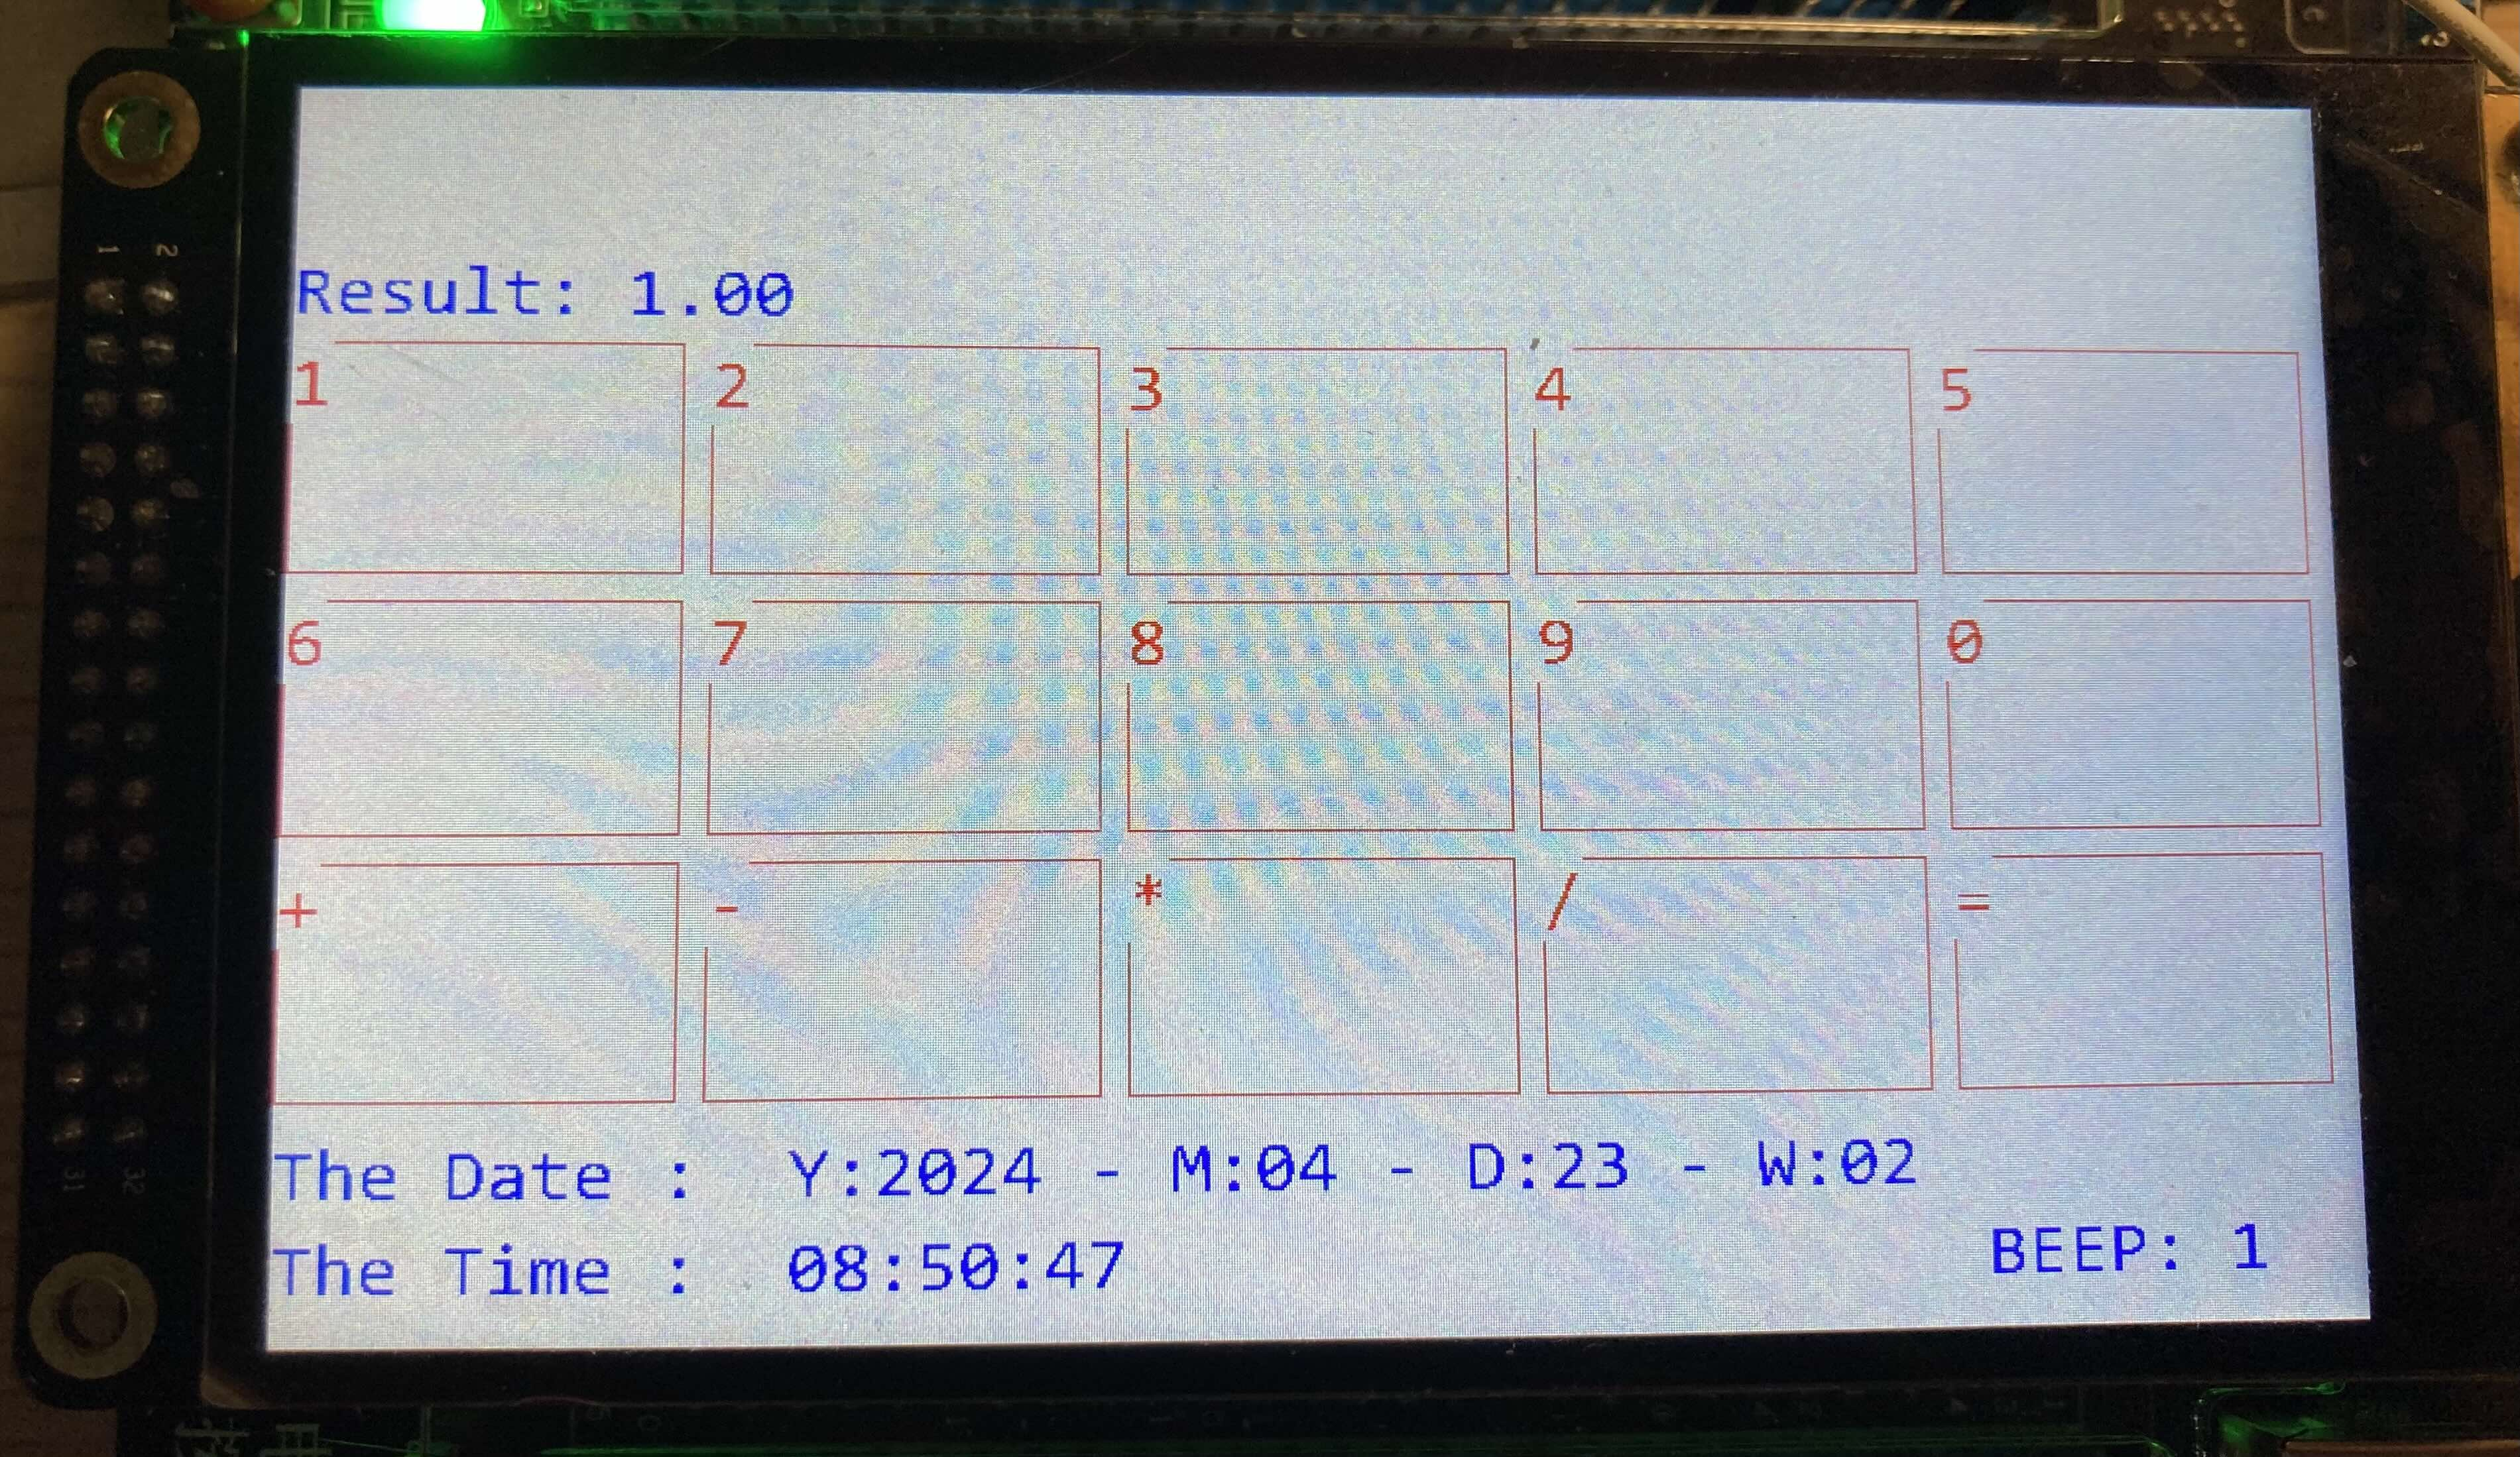
\includegraphics[width=0.6\linewidth]{start.jpg}
  \caption{启动}
\end{figure}

加法运算示例:

\begin{figure}[H]
  \centering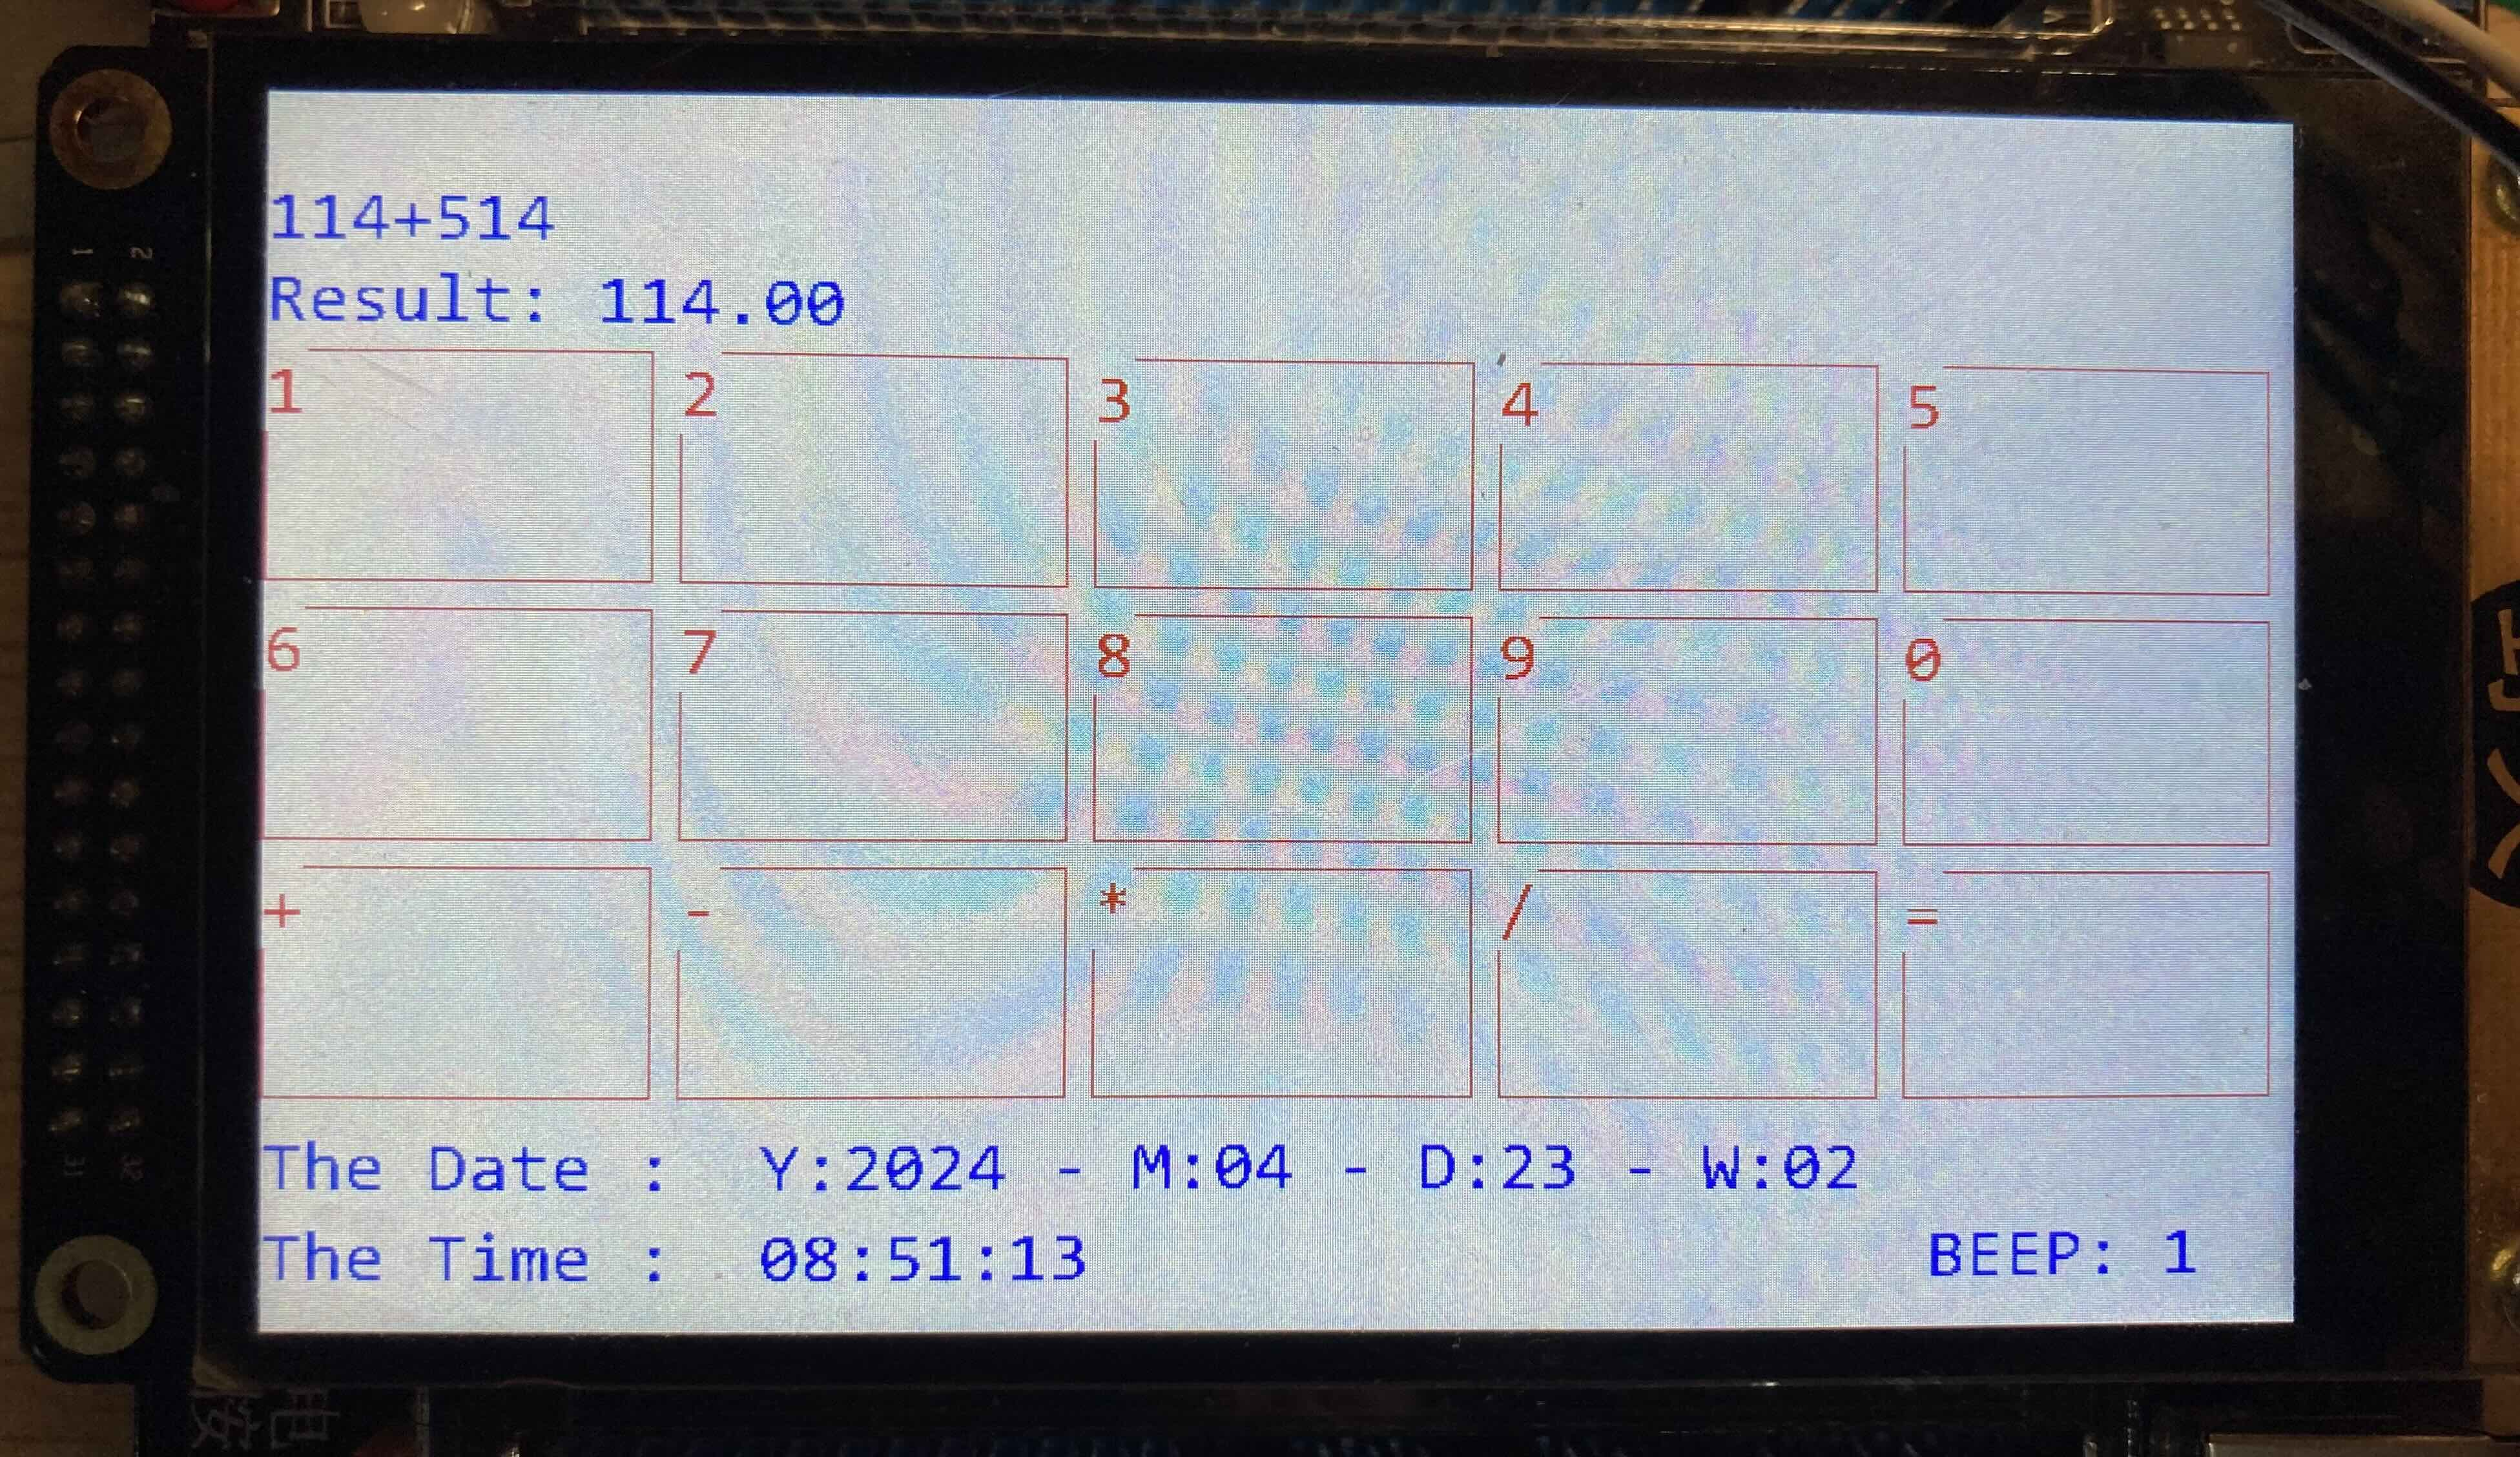
\includegraphics[width=0.6\linewidth]{add-input.jpg}
  \caption{加法运算输入示例}
\end{figure}

\begin{figure}[H]
  \centering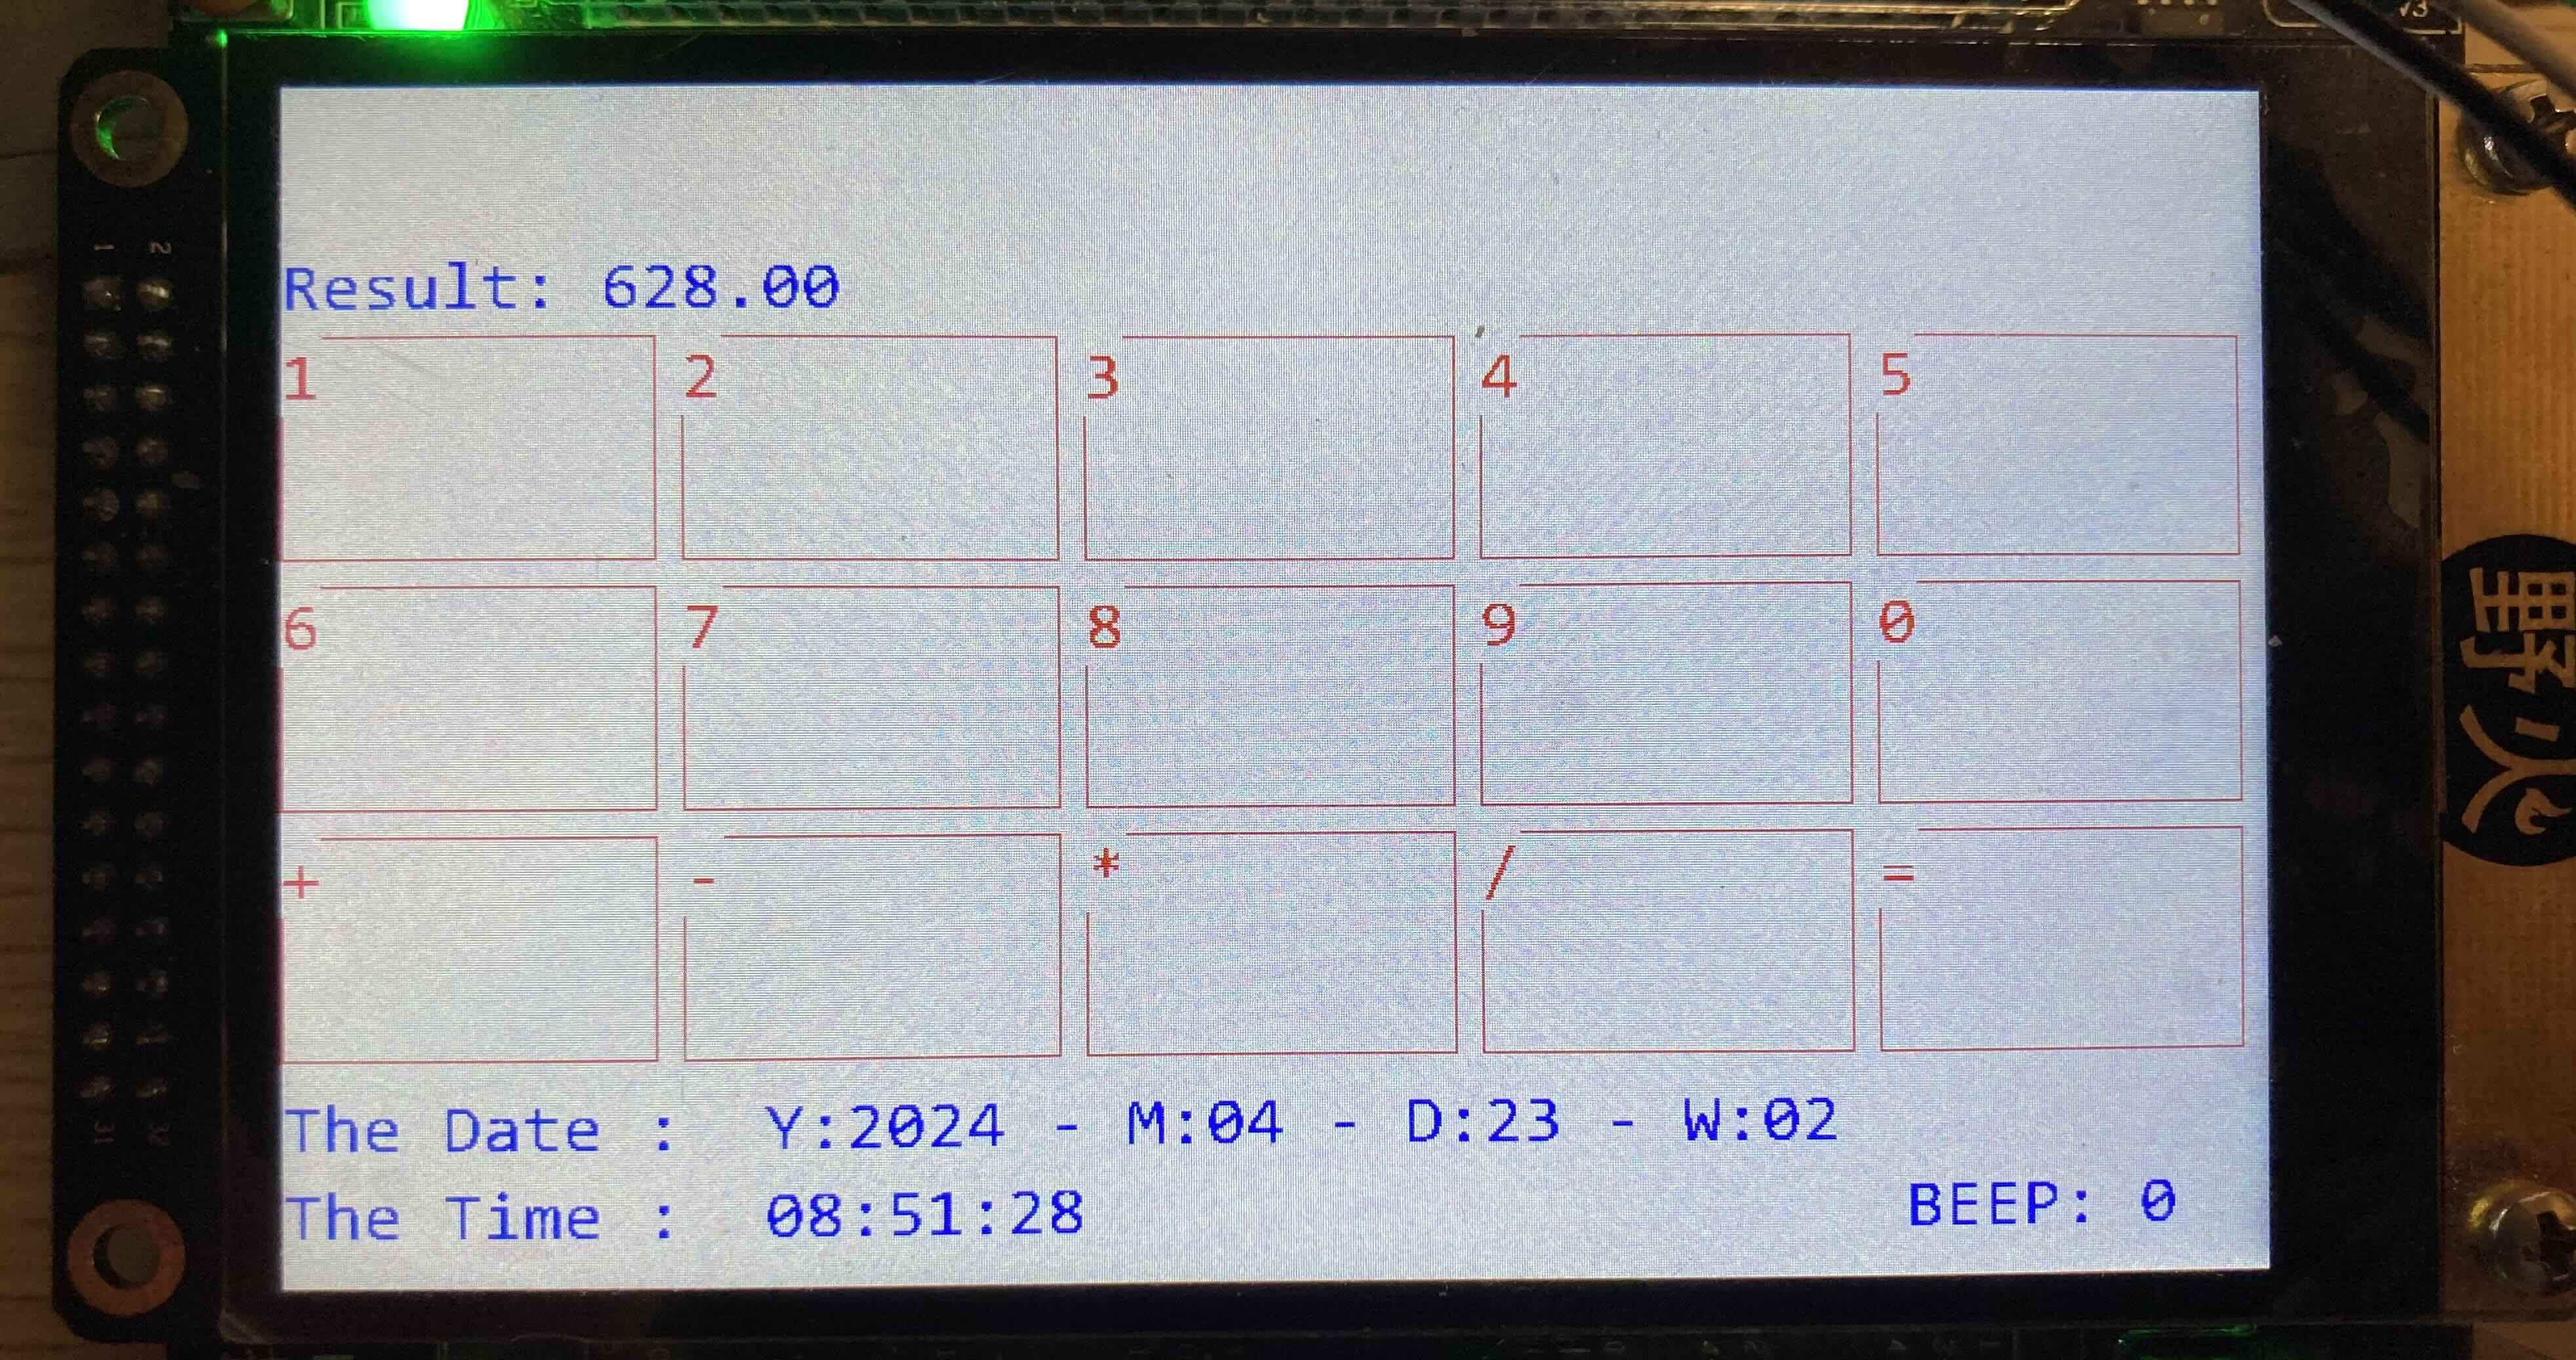
\includegraphics[width=0.6\linewidth]{add-result.jpg}
  \caption{加法运算结果}
\end{figure}

除法运算示例,将运算结果保留两位小数:

\begin{figure}[H]
  \centering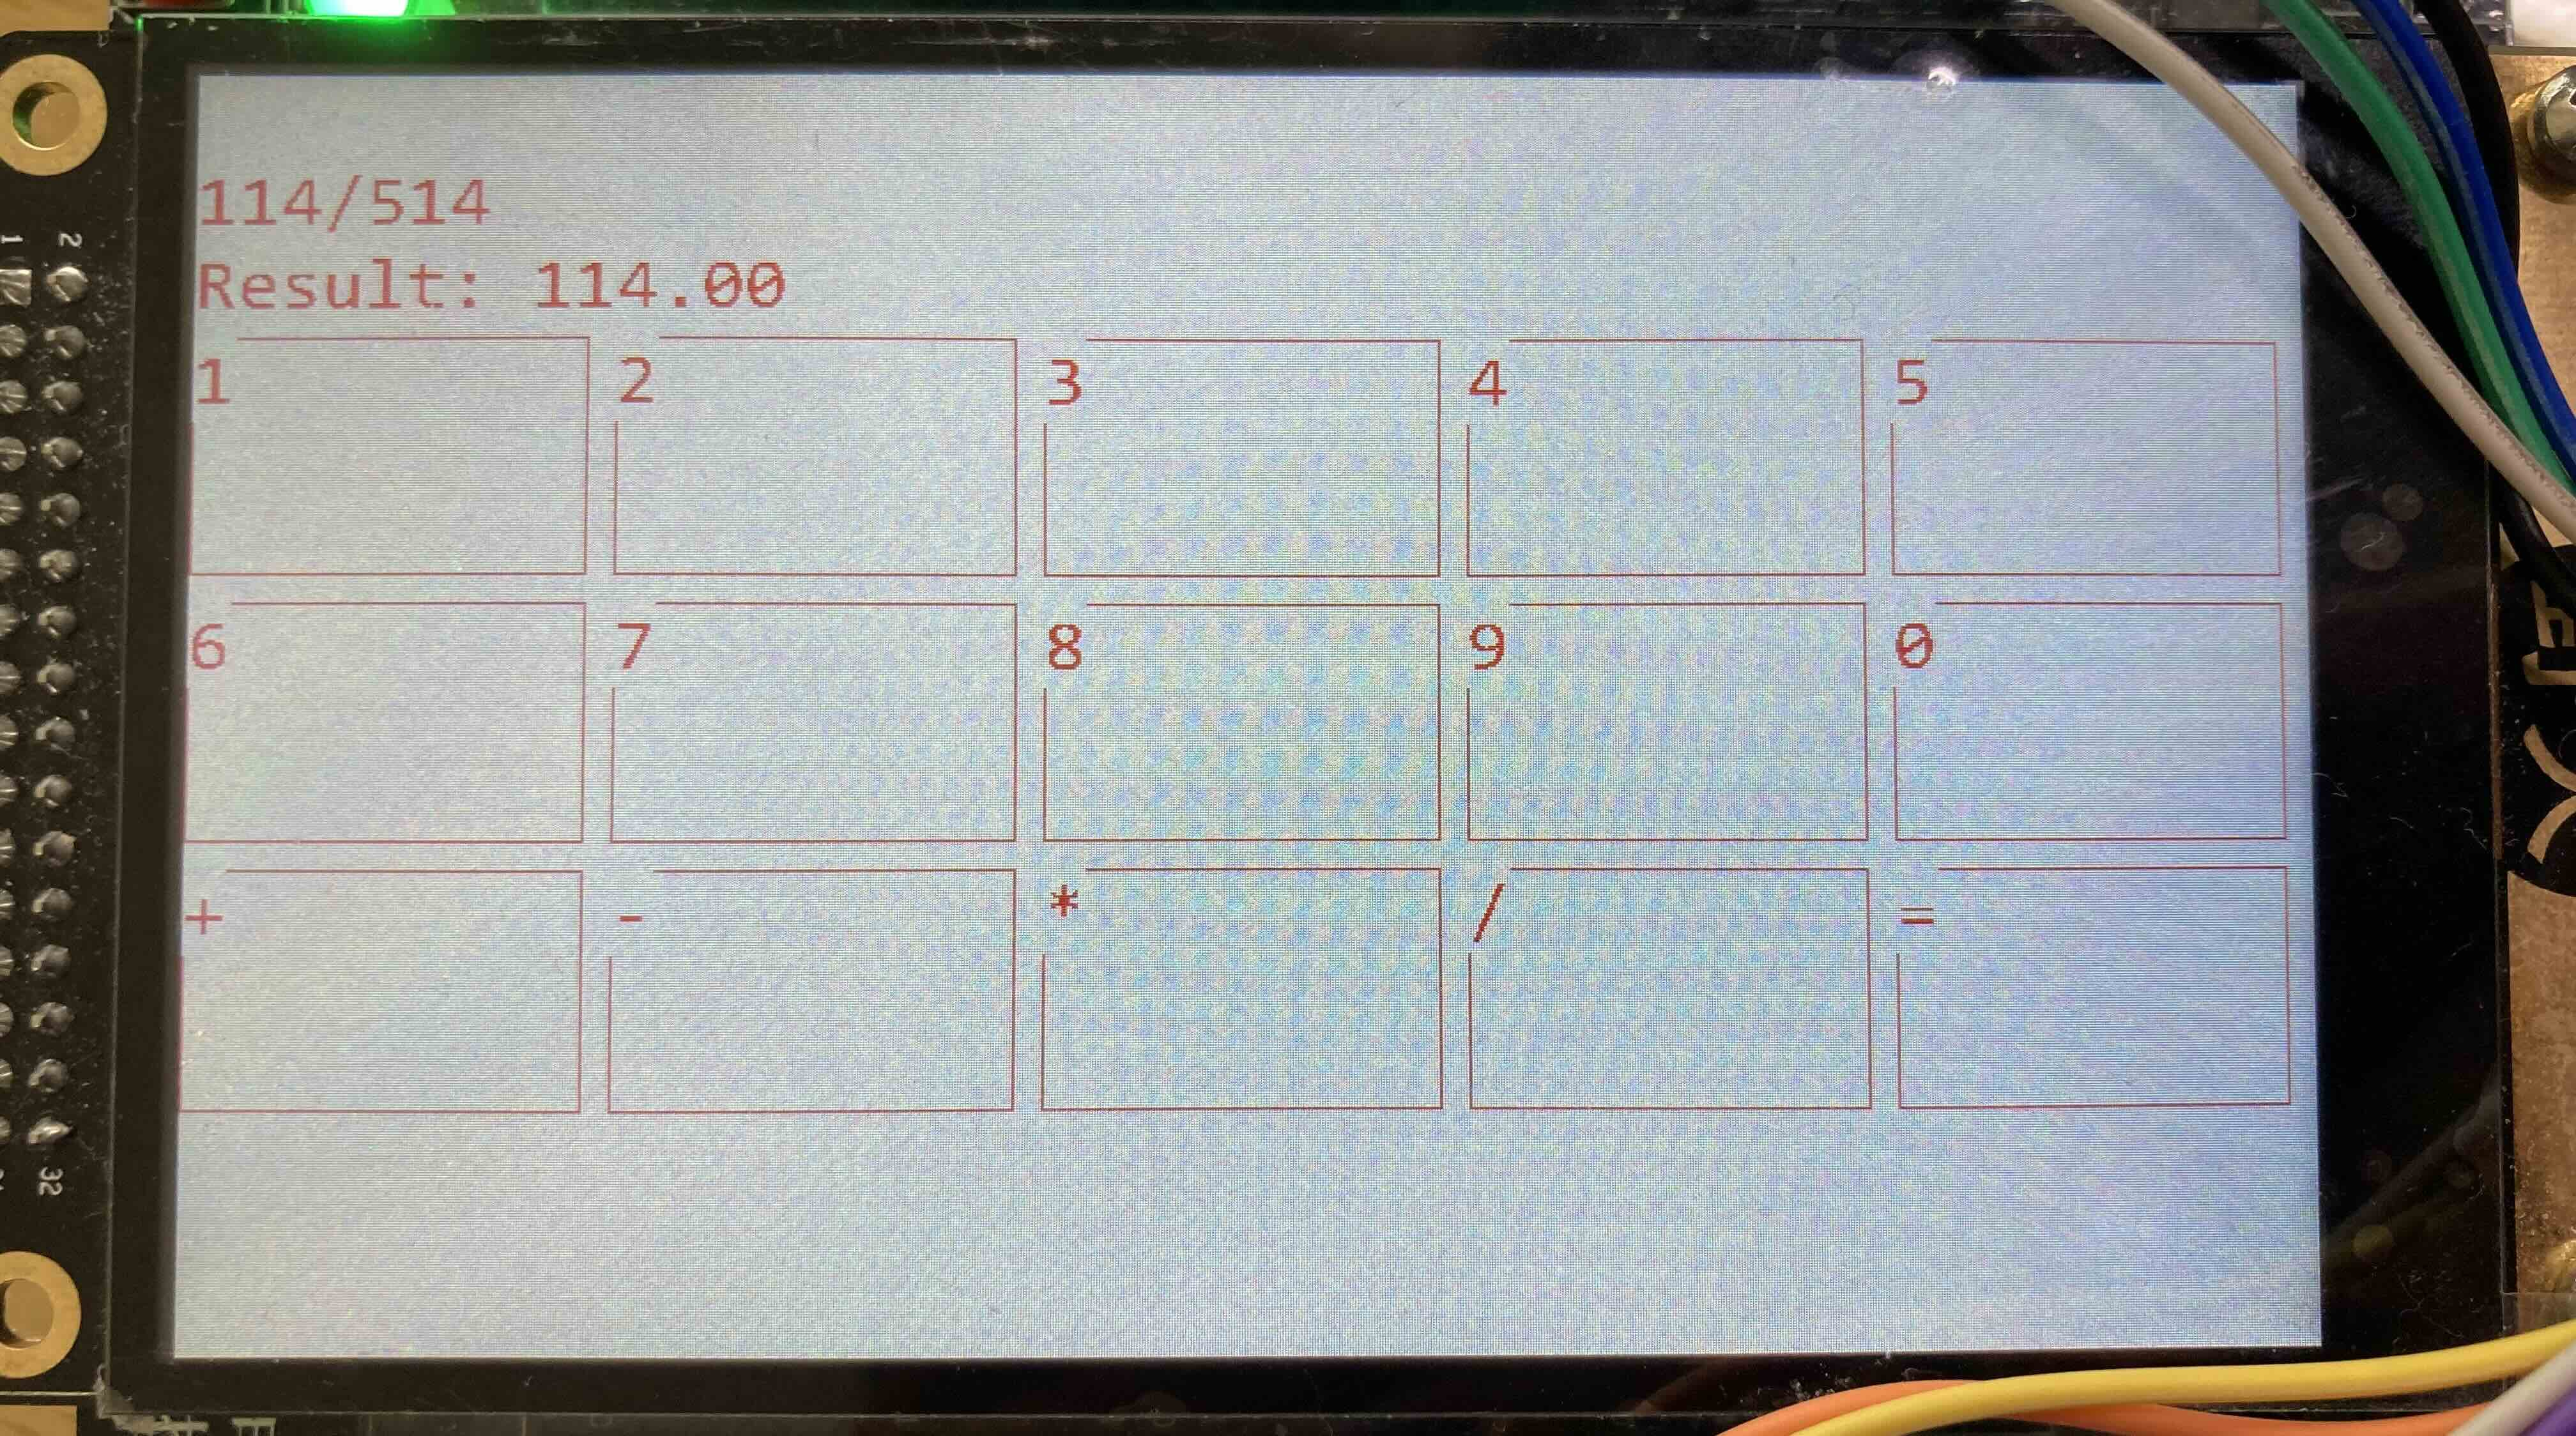
\includegraphics[width=0.6\linewidth]{division-input.jpg}
  \caption{除法运算输入示例}
\end{figure}

\begin{figure}[H]
  \centering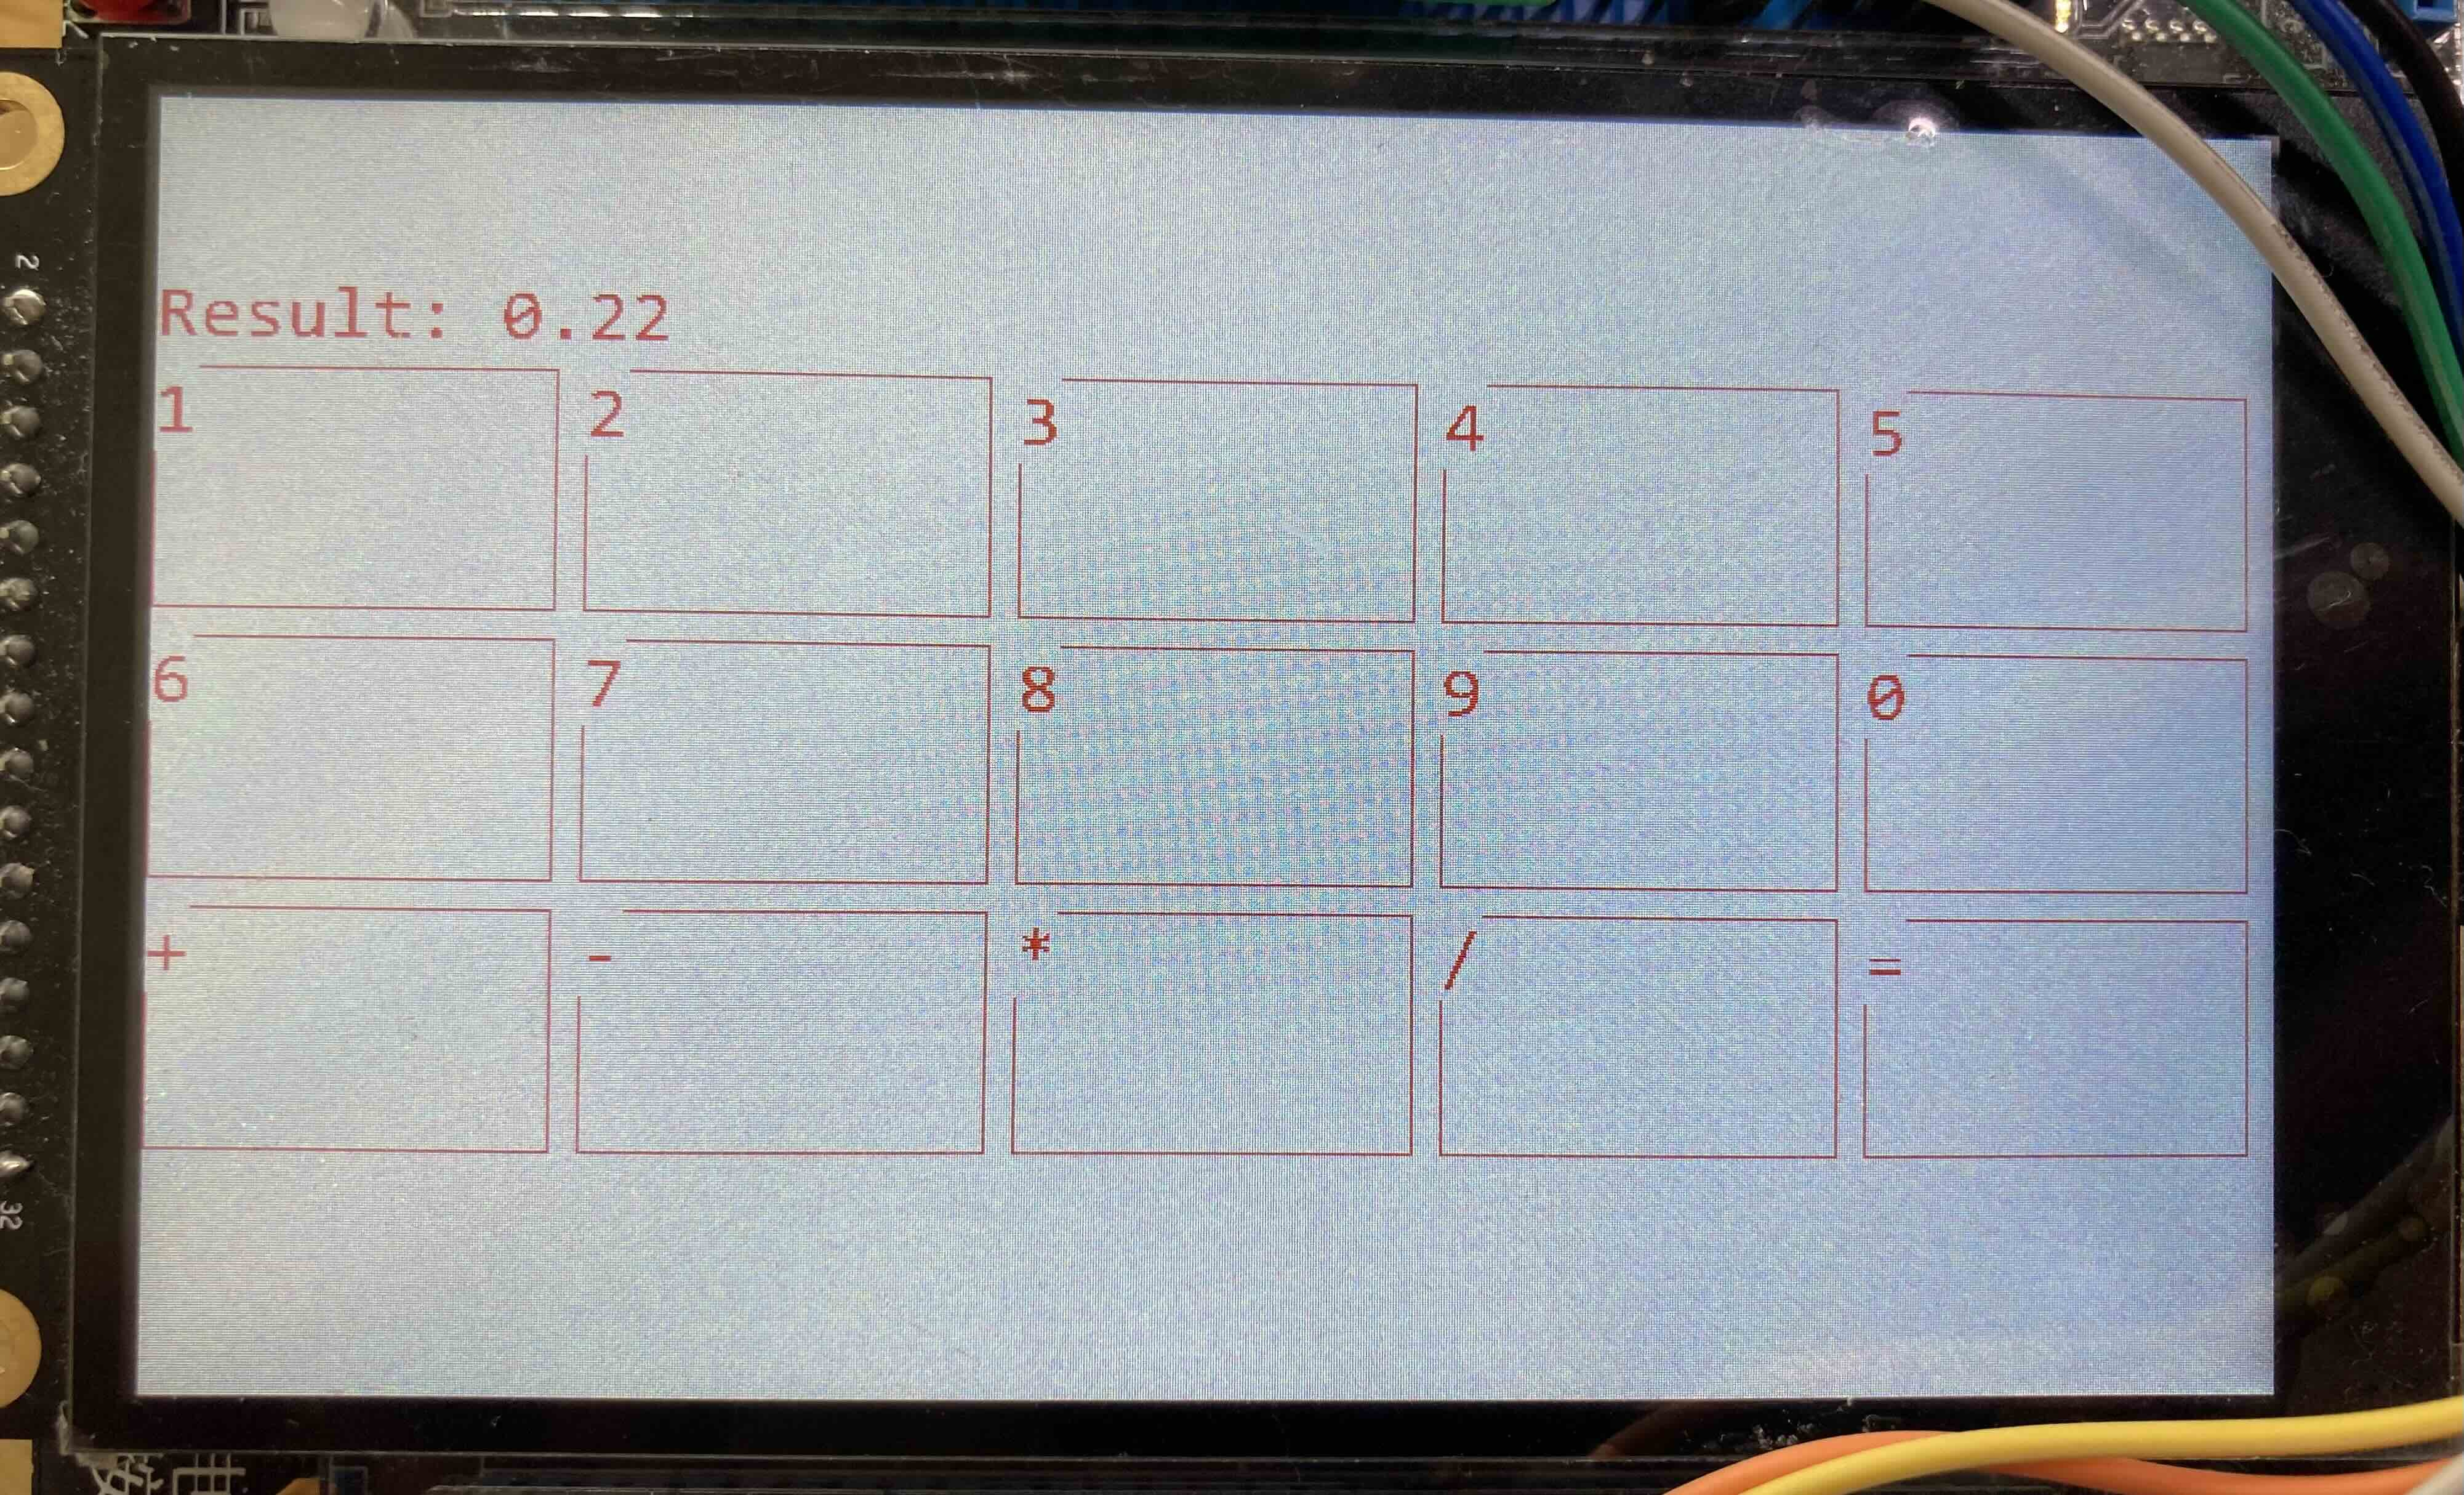
\includegraphics[width=0.6\linewidth]{division-result.jpg}
  \caption{除法运算结果}
\end{figure}

\section{总结}

通过本次实验,我学会了如何使用 STM32F4 微控制器,结合触摸屏、键盘、蜂鸣器等外设,实现一个简易的计算器。
对 STM32F4 微控制器的使用有了更深入的了解,对触摸屏的使用也有了更多的实践经验。
通过本次实验,我对嵌入式系统的开发有了更深入的了解,对嵌入式系统的开发有了更多的实践经验。

\end{document}
